\documentclass[11pt,reqno]{amsart}
\usepackage[margin=2.4cm]{geometry}
\usepackage{amsmath,amssymb}
\usepackage[final]{microtype}
\usepackage{booktabs}
\usepackage{tikz}
\usepackage{xcolor}
\definecolor{linkblue}{rgb}{0.0,0.2,0.55}
\usepackage[colorlinks=true,linkcolor=linkblue,citecolor=linkblue,urlcolor=linkblue]{hyperref}
\hypersetup{pdftitle={Riordan lattice paths counted by area},pdfauthor={Ilmar Gahramanov}}
\numberwithin{equation}{section}

\newtheorem{theorem}{Theorem}[section]
\newtheorem{proposition}[theorem]{Proposition}
\newtheorem{corollary}[theorem]{Corollary}
\newtheorem{lemma}[theorem]{Lemma}
\theoremstyle{remark}
\newtheorem{remark}[theorem]{Remark}

\newcommand{\area}{\operatorname{area}}
\newcommand{\qb}[2]{\genfrac{[}{]}{0pt}{}{#1}{#2}_{q}}

\title[Riordan lattice paths counted by area]{Riordan lattice paths counted by area}
\author[Ilmar Gahramanov]{Ilmar Gahramanov$^{1,2}$}
% affiliations and e-mail are printed below the author name on the first page;
% the amsart end-of-paper address block is suppressed
\makeatletter
\def\@setaddresses{}
\g@addto@macro\@setauthors{%
  \par\vspace{6pt}%
  {\centering\normalfont\small
   $^{1}$Department of Physics, Bo\u{g}azi\c{c}i University, 34342 Bebek, Istanbul, T\"urkiye\par
   \vspace{2pt}%
   $^{2}$Department of Mathematics, Khazar University, 41 Mehseti St., AZ1096 Baku, Azerbaijan\par
   \vspace{6pt}%
   E-mail: {\hypersetup{urlcolor=black}\href{mailto:ilmar.gahramanov@bogazici.edu.tr}{\texttt{ilmar.gahramanov@bogazici.edu.tr}}}\par}%
}
\makeatother

\subjclass[2020]{Primary 05A15, 05A16; Secondary 33D15, 05A19, 60C05, 16G20}
\keywords{Lattice path, Motzkin path, Riordan path, area statistic, $q$-series, continued fraction, Rogers-Ramanujan identities, quiver generating series, limit law}

\begin{document}

\begin{abstract}
We study Riordan paths enumerated by the area between the path and the axis. We show that the generating
function satisfies a $q$-Riccati equation and can be written in a closed form as a ratio
of basic hypergeometric series. The auxiliary series admits an algebraic representation as
the motivic generating series of a symmetric two-node quiver. We obtain explicit formulas
for the coefficients, the exponential asymptotics of the number of paths of given area,
and a linear recurrence whose coefficients are signed counts of partitions into distinct
parts. For a random path of area $n$ we obtain a joint Gaussian limit law for the numbers
of returns, horizontal steps and up steps. The height is of order $\sqrt{\log n}$ and
concentrates on two adjacent integers, which we determine explicitly.
\end{abstract}

\maketitle

\section{Introduction}

Lattice paths weighted by area appear in polymer and
vesicle models \cite{OP12,Poly22}, in the study of exclusion statistics and Hofstadter-type
Hamiltonians \cite{Gan25,GOP22,OP21}, and in knot
theory.\footnote{Let us also mention that Motzkin paths and Motzkin polynomials appear in
integrable Hamiltonian systems arising from the exact renormalization group flow in matrix
scalar field theory, where the conserved quantities are labelled by lattice paths
\cite{GM20}; see \cite{AM26,Mul23} for further developments in this direction.} Namely,
in the so-called knots-quivers correspondence \cite{KRSS19,PSS18,SS25} certain families of
paths below lines of rational slope encode coloured HOMFLY-PT invariants of torus knots.
For several directed-path models, $q$-difference equations and quotients of $q$-series
provide a useful description of the generating functions. For further developments in
the knot-theoretic direction see \cite{DS24,DP26,JTY24,Stosic24} and the review \cite{KN25}.

In this paper we study Riordan paths at fixed area. Recall that a \emph{Motzkin path} of
length $n$ runs from $(0,0)$ to $(n,0)$ with steps $U=(1,1)$, $D=(1,-1)$ and $H=(1,0)$
and never passes below the $x$-axis. A \emph{Riordan path} is a Motzkin path with no
horizontal steps on the axis, and a \emph{Dyck path} has no horizontal steps at all.
Enumeration by length gives the Riordan numbers $1,0,1,1,3,6,15,36,91,\dots$ and the
Catalan numbers, respectively. Here we instead fix the area between the path and the
axis, and we assign the weight $x$ to each up step and the weight $y$ to each horizontal
step.

Let us mention that length-area generating functions for Motzkin meanders with boundary
markers were obtained by Polychronakos \cite{Poly22}; setting the weight of horizontal
steps on the floor to zero in his formulas gives the Riordan case. Counts with prescribed
step profiles were also studied by Gan, Ouvry and Polychronakos \cite{GOP22}. Here we use
these path decompositions to study the fixed-area ensemble. We give explicit coefficient
formulas and a partition recurrence, and determine the exponential growth, additive
statistics and height distribution at large area. We also express the auxiliary
$q$-series as the generating series of a symmetric two-node quiver; this is an algebraic
identity, without an associated knot invariant.

Let $S_n(x,y)$ be the weight polynomial of the paths of area $n$ and let
$F(x,y;q)=\sum_{n\ge0}S_n(x,y)q^n$. As the point of departure one may regard the
following functional equation,
\begin{equation}\label{eq:intro-fe}
F(x,y;q)-1=q\,F(xq^2,yq;q)\,\big[(x+y)F(x,y;q)-y\big],
\end{equation}
which follows from a decomposition of the path at its first horizontal step at height one
or its first return to the axis. The substitutions $x\mapsto xq^2$ and $y\mapsto yq$
account for the area gained when a path is lifted by one level. A continued fraction
expansion then leads to the closed form
\begin{equation}\label{eq:intro-closed}
F(x,y;q)=\frac{A(q)}{A(q)-xq\,A(q^2)},\qquad
A(z)=\sum_{n=0}^{\infty}\frac{(-1)^nq^{\binom n2}p_n(x,y;q)}{(q;q)_n}\,z^n,
\end{equation}
where $p_n$ stand for homogeneous forms of the Rogers continuous $q$-Hermite polynomials,
defined in Section~\ref{sec:closed}. Here and below we use the standard notation
\[
(a;q)_n=(1-a)(1-aq)\cdots(1-aq^{n-1}),\qquad (a;q)_\infty=\prod_{j\ge0}(1-aq^j),
\]
with $(a;q)_0=1$ and $|q|<1$. The identity \eqref{eq:intro-closed} holds as a formal
power series in $q$, and the quotient also gives the meromorphic continuation of $F$ to
the unit disc. For $y=0$ it reduces to the Rogers-Ramanujan type formula for Dyck paths
counted by area \cite{Flajolet80,FS09}. After the substitution $x=\alpha\beta$,
$y=\alpha+\beta$, the series $A$ turns out to be the motivic generating series of the
quiver with adjacency matrix $\left(\begin{smallmatrix}1&1\\1&1\end{smallmatrix}\right)$.
This allows one to compare \eqref{eq:intro-closed} with the quiver-series expressions for
area-weighted Schr\"oder paths \cite{PSS18,SS25}, although by itself it does not give a
knot interpretation of Riordan paths.

The rest of the paper is organized as follows. In Section~\ref{sec:def} we define the area
polynomials and list the first examples. In Section~\ref{sec:fe} we prove the functional
equation \eqref{eq:intro-fe} and derive a recurrence for the polynomials $S_n$. In
Section~\ref{sec:closed} we obtain the continued fraction and the closed form
\eqref{eq:intro-closed}, including the case of bounded height. In Section~\ref{sec:coef}
we give explicit formulas for the coefficients in terms of path profiles. In
Section~\ref{sec:asym} we derive the asymptotics of the number of paths and a linear
recurrence with partition-theoretic coefficients. In Section~\ref{sec:limit} we study the
limit laws of additive statistics and of the height. We conclude with remarks and open
problems.\footnote{Finite checks compare the polynomial recurrence and profile formula
with direct enumeration through area $16$, and the partition recurrence with step-by-step
counts through area $1500$. The Gaussian constants were evaluated independently and
compared with exact moments at area $300$; the height probabilities in
Table~\ref{tab:height} were also recomputed from exact counts. These checks complement
the proofs below.}

\section{Riordan paths and area polynomials}\label{sec:def}

In this section we fix the notation and state the problem. Let us first explain how the
area of a path is computed. A step from height $h$ to height $h'$ contributes $(h+h')/2$
to the area. In other words, an up or down step between heights $h$ and $h+1$ contributes
$h+\tfrac12$, while a horizontal step at height $h$ contributes $h$. Note that the total
area is an integer, since the numbers of up and down steps are equal. Every allowed step
contributes at least $\tfrac12$, so a Riordan path of area $n$ has length at most $2n$,
and in particular there are only finitely many such paths.\footnote{This is the reason
for excluding horizontal steps on the axis: a Motzkin path may contain arbitrarily many
of them without changing the area.} For $n\ge1$ we define
\begin{equation}
S_n(x,y)=\sum_{\area(P)=n}x^{\#U(P)}\,y^{\#H(P)},\qquad S_0=1,
\end{equation}
where the sum runs over Riordan paths of area $n$, and $\#U(P)$ and $\#H(P)$ stand for the
numbers of up and horizontal steps of $P$. A path with $i$ up steps and $j$ horizontal
steps has weight $x^iy^j$ and length $2i+j$. One can easily compute the first polynomials,
\begin{gather*}
S_1=x,\qquad S_2=x^2+xy,\qquad S_3=x^3+2x^2y+xy^2,\qquad S_4=x^4+3x^3y+3x^2y^2+xy^3+x^2,\\
S_5=x^5+4x^4y+6x^3y^2+4x^2y^3+xy^4+2x^3+2x^2y,
\end{gather*}
and $S_6,\dots,S_{10}$ are listed in Appendix~\ref{app:poly}. For instance, the path
$UHUDD$ in Figure~\ref{fig:path} has area $5$ and weight $x^2y$; it is one of the two
paths giving the term $2x^2y$ of $S_5$. The numbers $r_n=S_n(1,1)$ of Riordan paths of
area $n$ are, starting at $n=1$,
\begin{equation}\label{eq:rn}
1,\ 2,\ 4,\ 9,\ 20,\ 45,\ 101,\ 227,\ 511,\ 1150,\ 2589,\ 5829,\ 13124,\ 29550,\ \dots
\end{equation}
with $r_0=1$. The Dyck sequence $S_n(1,0)$ begins, for $n\ge1$, with
$1,1,1,2,3,4,6,9,14,21,\dots$ and is recorded as OEIS~A143951
\cite{OEIS}.\footnote{Let us mention that enumeration at fixed area differs from the total
area of all paths of a fixed length, which was studied in \cite{Bu23,Merlini03}.}

\begin{figure}[htb]
\centering
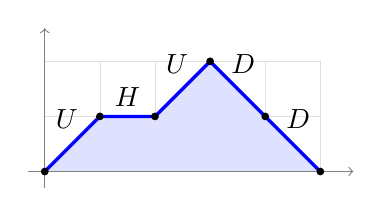
\begin{tikzpicture}[scale=0.7]
  \draw[gray!25,very thin] (0,0) grid (5,2);
  \fill[blue!12] (0,0)--(1,1)--(2,1)--(3,2)--(4,1)--(5,0)--cycle;
  \draw[->,gray] (-0.3,0)--(5.6,0); \draw[->,gray] (0,-0.3)--(0,2.6);
  \draw[very thick,blue] (0,0)--(1,1)--(2,1)--(3,2)--(4,1)--(5,0);
  \foreach \p in {(0,0),(1,1),(2,1),(3,2),(4,1),(5,0)} \fill \p circle (2pt);
  \node[above] at (0.4,0.6) {$U$}; \node[above] at (1.5,1) {$H$}; \node[above] at (2.4,1.6) {$U$};
  \node[above] at (3.6,1.6) {$D$}; \node[above] at (4.6,0.6) {$D$};
\end{tikzpicture}
\caption{The path $UHUDD$, of area $\tfrac12+1+\tfrac32+\tfrac32+\tfrac12=5$.}
\label{fig:path}
\end{figure}

\section{The functional equation}\label{sec:fe}

In this section we derive the functional equation \eqref{eq:intro-fe}. The key observation
is very simple. If one lifts a path by one level, every step gains area $1$, so the area
increases by the length of the path. Since a path of weight $x^iy^j$ has length $2i+j$,
the lift is represented by the substitution $x\mapsto xq^2$, $y\mapsto yq$. In what
follows we write $F^{\uparrow}=F(xq^2,yq;q)$.

\begin{theorem}\label{thm:fe}
The generating function satisfies
\begin{equation}\label{eq:fe}
F-1=q\,F^{\uparrow}\big[(x+y)F-y\big].
\end{equation}
For $x\ne0$ this can be rearranged as
\[
F(xq^2,yq;q)=\frac{F(x,y;q)-1}{q\,[(x+y)F(x,y;q)-y]},
\]
with the factor $q$ cancelled formally. At $x=0$ one has $F=1$, and the undivided
identity remains valid.
\end{theorem}

\begin{proof}
A nonempty Riordan path starts with $U$. Let us read it up to the first subsequent step
which either returns to the axis or is horizontal at height $1$. The segment $\hat R$ in
between is a Riordan path lifted by one level and contributes $F^\uparrow$. If the
distinguished step is $D$, one has $P=U\hat RDP'$ with an arbitrary Riordan path $P'$,
which contributes $xqF^\uparrow F$. If the distinguished step is $H$, one has
$P=U\hat RHW$, and removing $\hat RH$ leaves the nonempty Riordan path $UW$; this case
contributes $yqF^\uparrow(F-1)$. Adding the two contributions one obtains \eqref{eq:fe}.
\end{proof}

For nonzero $x$, \eqref{eq:fe} is an equation of $q$-Riccati type: the lifted function
$F^\uparrow$ is a linear fractional transform of $F$. For $y=0$ it reduces to the
equation $F=1+xqF(xq^2)F$ for Dyck paths counted by area, which goes back to Flajolet
\cite{Flajolet80}, see also \cite{OP12,FS09}; the Motzkin analogue was obtained by
Polychronakos \cite{Poly22}.\footnote{If one allows horizontal steps on the axis with
weight $z$, the generating function becomes $F/(1-zF)$, since such steps separate Riordan
components and contribute no area.}

Extracting the coefficient of $q^n$ in \eqref{eq:fe} one obtains the following recurrence
for the area polynomials,
\begin{equation}\label{eq:rec}
S_n=[t^{\,n-1}]\Big(\sum_{m<n}t^m\,S_m(xt^2,yt)\Big)\Big((x+y)\sum_{p<n}t^p\,S_p(x,y)-y\Big),
\qquad n\ge1 .
\end{equation}
For example, the first factor is $1+xt^3+\cdots$ and the second one is
$x+x(x+y)t+x(x+y)^2t^2+x(x+y)^3t^3+\cdots$, so that $S_4=x(x+y)^3+x^2$. Actually, the
substitution $S_m(xt^2,yt)$ retains the information about the length, which is needed for
the lift, and as a result \eqref{eq:rec} does not close on the numbers $r_n$ alone. A
scalar recurrence for $r_n$ will be given in Theorem~\ref{thm:rrec}.

\section{Continued fraction and closed form}\label{sec:closed}

In this section we obtain the continued fraction expansion of $F$ and, from it, the
closed form \eqref{eq:intro-closed}; we only need the simplest ingredients of the approach
of Flajolet \cite{Flajolet80}. Let $M_h$ be
the generating function of Motzkin paths based at height $h\ge1$, with the area measured
from the $x$-axis. Such a path is a sequence of horizontal steps and excursions above
height $h$, and therefore
$M_h=1/(1-yq^h-xq^{2h+1}M_{h+1})$ and $F=1/(1-xqM_1)$. In other words,
\begin{equation}\label{eq:cf}
F=\cfrac{1}{1-\cfrac{xq}{1-yq-\cfrac{xq^3}{1-yq^2-\cfrac{xq^5}{1-yq^3-\cdots}}}}\;.
\end{equation}

\subsection{Paths of bounded height}
Let us first look at the convergents of \eqref{eq:cf}. Truncating the continued fraction
at level $k\ge1$ one obtains the generating function $F^{[k]}$ of paths of height at most
$k$; for $k=0$ one has $F^{[0]}=1$. We write $F^{[k]}=R^{(k)}_1/R^{(k)}_0$, where
\begin{equation}\label{eq:R}
R^{(k)}_{k+1}=1,\qquad R^{(k)}_k=1-yq^k,\qquad
R^{(k)}_h=(1-yq^h)R^{(k)}_{h+1}-xq^{2h+1}R^{(k)}_{h+2}\quad(0\le h<k),
\end{equation}
with the factor $1-yq^0$ replaced by $1$ at $h=0$. Expanding this recurrence one recovers
the standard interpretation of the convergents in terms of matchings, which also goes
back to \cite{Flajolet80}. Namely, $R^{(k)}_h$ is the generating polynomial of
monomer-dimer configurations on the path graph with vertices $h,\dots,k$, where a monomer
on the vertex $v$ has weight $-yq^v$ and a dimer on the edge $\{v,v+1\}$ has weight
$-xq^{2v+1}$.\footnote{No monomer is allowed on the vertex $0$, which reflects the absence
of horizontal steps on the axis.} Since every occupied vertex $v$ contributes $q^v$, one
can write, for $1\le h\le k$,
\begin{equation}\label{eq:match}
R^{(k)}_h=\sum_{S\subseteq\{h,\dots,k\}}q^{\sum S}\prod_{I}m_{|I|}(x,y),
\qquad m_r(x,y)=\sum_{d=0}^{\lfloor r/2\rfloor}\binom{r-d}{d}(-x)^d(-y)^{r-2d},
\end{equation}
where the product runs over the maximal runs $I$ of consecutive integers in $S$, and
$m_r$ stands for the matching polynomial of the path with $r$ vertices. At the boundary
$h=0$ we use $R^{(k)}_0=R^{(k)}_1-xqR^{(k)}_2$. Equivalently, in the subset formula the run
containing $0$, if present, has weight $b_1=0$ and $b_r=-x\,m_{r-2}(x,y)$ for $r\ge2$,
since the vertex $0$ must be covered by the dimer $\{0,1\}$.

Two special cases can be written in a closed form. The dimer-only part, valid also at
$h=0$, is a $q^2$-binomial sum,
\[
R^{(k)}_h\big|_{y=0}=\sum_{m=0}^{\lfloor(k-h+1)/2\rfloor}(-x)^mq^{m(2m+1)+2m(h-1)}\genfrac{[}{]}{0pt}{}{k-h+1-m}{m}_{q^2},
\]
which at $h=1$ agrees with the formula obtained by Owczarek and Prellberg for Dyck paths
of bounded height \cite{OP12}. The monomer-only part is $(yq^h;q)_{k-h+1}$ for $h\ge1$ and
$(yq;q)_k$ for $h=0$. It seems that the mixed contributions do not factor in a similar
way.

At $x=y=1$ the exponential growth rate of the number of paths of height at most $k$ is
$1/q^{(k)}_0$, where $q^{(k)}_0$ denotes the smallest positive zero of $R^{(k)}_0$. One
finds
\[
1/q^{(k)}_0=2,\quad 2.2469796\ldots,\quad 2.2516428\ldots,\quad 2.2516611\ldots\qquad(k=1,2,3,4).
\]
Paths of height one contribute $x(x+y)^{n-1}$ at area $n\ge1$, which explains the first
value. For height at most two, $1/q^{(2)}_0=1+2\cos(2\pi/7)$ is the largest root of
$t^3-2t^2-t+1$. The rapid convergence to the limit $1/q_0=2.2516612\ldots$ is a curious
phenomenon, which will be explained in Theorem~\ref{thm:height}.

\subsection{The closed form}
Let us now take $k\to\infty$. For each fixed $h\ge1$ one finds from \eqref{eq:R} that
$R^{(k)}_h\to A(q^h)$, where
\begin{equation}\label{eq:Afe}
A(z)=(1-yz)A(zq)-xqz^2A(zq^2),\qquad A(0)=1 .
\end{equation}
We usually suppress the dependence on $x,y,q$ and write $A(z)$ for $A(z;x,y;q)$. At the
boundary one has $R^{(k)}_0\to A(q)-xqA(q^2)$. Comparing coefficients, the solution of
\eqref{eq:Afe} is the series $A$ in \eqref{eq:intro-closed}, where the polynomials $p_n$
are determined by
\begin{equation}\label{eq:pn}
p_0=1,\qquad p_1=y,\qquad p_n=y\,p_{n-1}-x(1-q^{n-1})\,p_{n-2}.
\end{equation}
Then $M_h=A(q^{h+1})/A(q^h)$ and $F=1/(1-xqM_1)=A(q)/(A(q)-xqA(q^2))$, which proves
\eqref{eq:intro-closed}. Equivalently, $1/F=y+A(1)/A(q)$.

\begin{lemma}\label{lem:analytic}
For fixed complex $x,y$, the series $A(z;x,y;q)$ is entire in $z$ and holomorphic in
$q$ for $|q|<1$. For each $h\ge1$, the continuants $R^{(k)}_h$ converge to $A(q^h)$
locally uniformly in this disc. In particular, \eqref{eq:intro-closed} defines a
meromorphic function of $q$ there.
\end{lemma}

\begin{proof}
Fix $0<r<1$. The recurrence \eqref{eq:pn} gives $|p_n|\le K^n$ for $|q|\le r$,
with $K$ depending only on $x,y$. Also
$|(q;q)_n|\ge\prod_{j\ge1}(1-r^j)>0$. The factor $q^{\binom n2}$ therefore ensures
local uniform convergence of the series for $A$ in $(z,q)$.

For the continuants, ignore the exclusion constraints in the matching expansion.
The sum of the absolute weights of all configurations on the infinite path is bounded by
\[
\prod_{v\ge h}\bigl(1+|y|r^v+|x|r^{2v+1}\bigr)<\infty.
\]
The weights of configurations involving vertices beyond $k$ tend to zero uniformly on
$|q|\le r$. Hence the finite continuants converge locally uniformly. Their formal limit,
already identified above, is $A(q^h)$. The denominator in \eqref{eq:intro-closed}
is holomorphic and equals $1$ at $q=0$, which proves the last assertion.
\end{proof}

\begin{remark}\label{rem:hermite}
Let us write $x=\alpha\beta$ and $y=\alpha+\beta$. Then the solution of \eqref{eq:pn}
takes the form
\[
p_n=\sum_{k=0}^n\qb nk\alpha^{n-k}\beta^k,
\]
which is a homogeneous form of the continuous $q$-Hermite polynomial of Rogers. Namely,
one has
$p_n=x^{n/2}H_n(y/(2\sqrt{x})\mid q)$ for $x\ne0$, with its polynomial extension at
$x=0$. Moreover, one can write
\[
A(z)=(\alpha z;q)_\infty\;{}_1\phi_1\!\left(\begin{matrix}0\\ \alpha z\end{matrix};\,q,\,\beta z\right),
\]
which is a $q$-Bessel type function, see e.g.\ \cite{GR04}. At apparent singularities
of the product representation, the identity is understood by analytic continuation.
\end{remark}

\begin{remark}[An algebraic quiver-series representation]\label{rem:quiver}
Let us introduce the so-called symmetric-quiver series
\[
P_C(x_1,x_2)=\sum_{d_1,d_2\ge0}
\frac{(-q^{1/2})^{d^TCd}x_1^{d_1}x_2^{d_2}}
{(q;q)_{d_1}(q;q)_{d_2}},\qquad
C=\begin{pmatrix}1&1\\1&1\end{pmatrix}.
\]
Since $d^TCd=(d_1+d_2)^2$ and $(-q^{1/2})^{n^2}=(-1)^nq^{n^2/2}$, grouping the terms with
$d_1+d_2=n$ one obtains the formal identities
\begin{equation}\label{eq:quiver}
A(z)=P_C\big(\alpha zq^{-1/2},\,\beta zq^{-1/2}\big),\qquad
\frac1F-y=\frac{P_C(\alpha q^{-1/2},\beta q^{-1/2})}{P_C(\alpha q^{1/2},\beta q^{1/2})}.
\end{equation}
Ratios of quiver series at $q$-shifted arguments occur in the enumeration of
area-weighted Schr\"oder paths \cite{PSS18,SS25}, where the corresponding $q$-difference
equations are related to the so-called quantum $A$-polynomials; combinatorial derivations
of such equations appear in \cite{JTY24}, and the coefficient formulas of \cite{DS24} may
be compared with Theorem~\ref{thm:profile} below. In the conventions of \cite{SS25}, the
Schr\"oder-path quiver of slope $1/f$ has the matrix
$\left(\begin{smallmatrix}f&f\\f&f+1\end{smallmatrix}\right)$, so that our matrix differs
from its $f=1$ case by one diagonal entry. For $y=0$ the specialization \eqref{eq:dyck}
below can similarly be written as $F(x,0;q)=P_{(2)}(-xQ^{1/2};Q)/P_{(2)}(-xQ^{-1/2};Q)$
with $Q=q^2$, and the one-node quiver $(2)$ appears in the formulas for the reduced
unknot in framing two \cite{SS25}. We stress that these are comparisons of formal series
and adjacency matrices, not of knot invariants.
\end{remark}

For $y=0$, i.e.\ $\beta=-\alpha$, the closed form becomes the Rogers-Ramanujan type
identity
\begin{equation}\label{eq:dyck}
F(x,0;q)=\frac{\sum_{k\ge0}(-x)^kq^{k(2k+1)}/(q^2;q^2)_k}{\sum_{k\ge0}(-x)^kq^{k(2k-1)}/(q^2;q^2)_k},
\end{equation}
in agreement with \cite{OP12,FS09}. Finally, taking $k\to\infty$ in \eqref{eq:match} one
obtains a second interpretation of the auxiliary series: for $h\ge1$, $A(q^h)$ enumerates
partitions into distinct parts at least $h$, with each maximal run of $r$ consecutive
parts weighted by $m_r(x,y)$. We will need this interpretation in Section~\ref{sec:asym}.

\section{Explicit formulas for the coefficients}\label{sec:coef}

In this section we give explicit formulas for the coefficients of $S_n$. Let us start
with a simple observation. Deleting the horizontal steps of a Riordan path leaves its
Dyck \emph{skeleton}. Conversely, one can insert an arbitrary run of horizontal steps at
each skeleton vertex $v$ of positive height $h(v)$. Each inserted step has weight
$yq^{h(v)}$, and therefore
\begin{equation}\label{eq:skel}
F=\sum_{D\ \mathrm{Dyck}}x^{\#U(D)}q^{\area(D)}\prod_{v}\frac1{1-yq^{h(v)}},
\end{equation}
where the product runs over the vertices of $D$ of positive height. For fixed $m$, the
coefficient $F_m=[x^m]F$ is a rational function of $q$ whose denominator divides
$\prod_{h=1}^m(1-yq^h)^{m+1-h}$. For example, $F_1=q/(1-yq)$ and
$F_2=\frac{q^2}{(1-yq)^2}+\frac{q^4}{(1-yq)^2(1-yq^2)}$. In particular, the paths of
height one contribute exactly $x(x+y)^{n-1}$ to $S_n$, which is the leading row visible
in Appendix~\ref{app:poly}.

In order to obtain a positive formula for all coefficients, we will need also the
following profiles. The Dyck skeleton count used below is the lowest-floor case of
\cite[Eq.~(18)]{GOP22}; that work also treats horizontal-step profiles. We include a
direct proof to make the fixed-area constraint explicit. For a path $P$, let $t_h$ be the number of its interior vertices at
height $h$, and let $u_h$ be the number of its up steps from height $h$ to $h+1$. Summing
the contributions of the endpoints of each step one finds
\begin{equation}\label{eq:vertex}
\area(P)=\sum_{h\ge1}h\,t_h,
\end{equation}
i.e.\ the area is the sum of the heights of the interior vertices. If $P$ has height $H$,
its up-profile $(u_0,\dots,u_{H-1})$ is a composition of $\#U(P)$, and its skeleton has
$v_h=u_{h-1}+u_h$ vertices at each height $1\le h\le H$, where $u_H=0$.

\begin{theorem}\label{thm:profile}
Let $u=(u_0,\dots,u_{H-1})$ be a composition and let $t=(t_1,\dots,t_H)$ be a sequence of
positive integers, and set $u_H=0$. Here a binomial coefficient is zero when its lower
argument exceeds its nonnegative upper argument. The number of Riordan paths with
up-profile $u$ and vertex profile $t$ is
\[
\prod_{h=1}^{H}\binom{u_{h-1}+u_h-1}{u_h}\binom{t_h-1}{u_{h-1}+u_h-1}.
\]
Consequently,
\[
F=1+\sum_{u}x^{|u|}\prod_{h=1}^{H}\binom{u_{h-1}+u_h-1}{u_h}\Big(\frac{q^h}{1-yq^h}\Big)^{u_{h-1}+u_h},
\]
where the sum runs over all nonempty compositions $u$ and $H$ denotes the number of parts.
For $m\ge1$, the number of paths of area $n$ with $m$ up steps and $j$ horizontal steps
is
\[
c(n,m,j)=\sum_{\substack{u\models m,\ t\\ \sum_ht_h=2m-u_0+j,\ \sum_hh\,t_h=n}}
\ \prod_{h=1}^{H}\binom{u_{h-1}+u_h-1}{u_h}\binom{t_h-1}{u_{h-1}+u_h-1}.
\]
\end{theorem}

\begin{proof}
Let us first count the Dyck skeletons with profile $u$. At level $h$, the $u_h$
excursions above height $h$ are distributed among the $u_{h-1}$ excursions rising from
height $h-1$. This is a weak composition into $u_{h-1}$ parts, counted by
$\binom{u_{h-1}+u_h-1}{u_h}$, and applying this construction at successive levels one
obtains the first factor.

Next, at height $h$, one distributes $t_h-v_h$ horizontal steps among the $v_h$ skeleton
vertices; there are $\binom{t_h-1}{v_h-1}$ choices, which gives the second factor. The
area is then determined by \eqref{eq:vertex}. Since the skeleton has $u_0$ primitive
components, exactly $u_0-1$ of its interior vertices lie on the axis, and therefore it
has $2m-u_0$ vertices of positive height. Inserting $j$ horizontal steps gives
$\sum_{h=1}^{H}t_h=2m-u_0+j$, which proves the formula for $c(n,m,j)$. Summing over the
insertions at each height one obtains the generating function, where the term $1$
represents the empty path.
\end{proof}

\section{Asymptotics and a linear recurrence}\label{sec:asym}

In this section we determine the growth of the numbers $r_n$ and obtain a recurrence for
them. The point of departure is the decomposition of a path into its \emph{primitive}
components, i.e.\ the pieces between consecutive returns to the axis. Every nonempty
Riordan path decomposes uniquely into primitive paths, which touch the axis only at their
endpoints. At $x=y=1$ their generating function is
\[
g(q)=\sum_{P\ \text{primitive}}q^{\area(P)}=q+q^2+q^3+2q^4+3q^5+5q^6+\cdots.
\]
Therefore $F(1,1;q)=1/(1-g)$ and, by \eqref{eq:intro-closed}, $g=qA(q^2)/A(q)$. Each
primitive component contributes one return to the axis, including the final one, so
marking the returns by $u$ one obtains $F(u;q)=1/(1-ug)=F/(u+(1-u)F)$.

\begin{theorem}\label{thm:asym}
Let $\rho$ be the radius of convergence of $g$. The equation $g(q)=1$ has a unique root
$q_0\in(0,\rho)$, which is also the smallest positive root of $A(q)=qA(q^2)$ at
$x=y=1$. For some $\theta<1$,
\[
r_n=C\,q_0^{-n}\big(1+O(\theta^n)\big),\qquad C=\frac{1}{q_0\,g'(q_0)},
\]
with
\[
q_0=0.44411654605086\ldots,\quad q_0^{-1}=2.25166121121160\ldots,\quad C=0.34315827064\ldots
\]
\end{theorem}

\begin{proof}
The series $g$ has nonnegative coefficients and a positive radius of convergence, since
a path of area $n$ has length at most $2n$. By Lemma~\ref{lem:analytic}, $g$ is
meromorphic in $|q|<1$. The primitive
paths $UH^jD$ give $g(t)\ge t/(1-t)$ wherever both sides converge, so $\rho\le1$. If
$\rho<1$, Pringsheim's theorem together with meromorphicity implies that $\rho$ is a pole
and $g(t)\to\infty$ as $t\uparrow\rho$. If $\rho=1$, the same divergence follows from the
lower bound. Since $g$ is strictly increasing on $[0,\rho)$, it reaches $1$ at a unique
point $q_0<\rho$.

For $|q|\le q_0$ one has $|g(q)|\le g(|q|)\le1$. On $|q|=q_0$, equality in the triangle
inequality requires the terms of degrees $1$ and $2$ to have the same argument, and their
positive coefficients force $q=q_0$. Thus $1-g$ has a unique zero in the closed disc, and
this zero is simple because $g'(q_0)>0$. Analyticity in a larger disc and isolation of
zeros give an exponentially smaller remainder after subtraction of the simple pole, and
the residue gives $C=1/(q_0g'(q_0))$.

It remains to rule out a cancellation in the quotient for $g$. Let us display the base
parameter of $A$ explicitly. If, for some $0<t<1$, both $A(t;1,1;t)$ and $A(t^2;1,1;t)$
vanished, the recurrence for $B_h=A(t^h;1,1;t)$,
\[
B_h=(1-t^h)B_{h+1}-t^{2h+1}B_{h+2},
\]
would force $B_h=0$ for every $h\ge1$, which contradicts $B_h\to A(0;1,1;t)=1$.
Consequently a zero of $A(t;1,1;t)$ cannot cancel in $g(t)$, so $A(t;1,1;t)>0$ for
$0\le t<\rho$. On this interval the denominator is $A(q)(1-g(q))$, and its first positive
zero is $q_0$.
\end{proof}

Let us make a few comments. The leading asymptotics is already accurate at modest area;
namely, $r_{22}/(Cq_0^{-22})=1+4.8722\cdot10^{-7}$. A further positive pole is found
numerically at $q_1=0.77091704183\ldots$, and the argument principle applied numerically
on the circles $|q|=0.6,\,0.7,\,0.8$ gives $1,1,2$ zeros of $A(q)-qA(q^2)$. These
computations suggest that any $\theta\in(q_0/q_1,1)$ is admissible in
Theorem~\ref{thm:asym}; we do not use this sharper, uncertified estimate. We do not know closed forms for
$q_0$ and $C$; the Dyck constants $q_D=0.6629014851\ldots$ and $C_D=0.3377611503\ldots$
recorded in OEIS~A143951 \cite{OEIS} are likewise only known numerically. For positive
weights $x,y$ the same argument applies whenever the primitive generating function reaches
$1$ strictly inside its radius of convergence, which holds near $(x,y)=(1,1)$.

\subsection{A recurrence for \texorpdfstring{$r_n$}{rn}}
Let us now come back to the partition interpretation of Section~\ref{sec:closed}. We write
$A(q)|_{x=y=1}=\sum_n\nu_nq^n$ and $A(q^2)|_{x=y=1}=\sum_n\nu'_nq^n$. Then $\nu_n$ counts
partitions of $n$ into distinct parts, with each maximal run of $r$ consecutive parts
weighted by $m_r(1,1)=\sum_d(-1)^{r-d}\binom{r-d}d$, and $\nu'_n$ counts the same
partitions with the additional restriction that every part is at least $2$. The run
weights turn out to be periodic, namely $m_r(1,1)=1,-1,0$ for $r\equiv0,1,2\pmod3$,
respectively. The following simple cancellation explains this periodicity.

\begin{lemma}\label{lem:invol}
Let us write a perfect monomer-dimer cover of the path with $r$ vertices as a word in the
letters $M$ and $D$, with sign $(-1)^{\#\text{letters}}$. The map exchanging a leading
$D$ with a leading $MM$, and fixing the words with neither prefix, is an involution which
reverses the sign on its nonfixed pairs. Its fixed points are the words $MDw$, together
with $M$ and the empty word. Hence $m_r(1,1)=m_{r-3}(1,1)$ for $r\ge3$, with the initial
values $1,-1,0$.
\end{lemma}

\begin{theorem}\label{thm:rrec}
Let $r_0=1$, set $\nu'_{-1}=0$, and let $d_n=\nu_n-\nu'_{n-1}$ for $n\ge0$. Then
\[
r_n=\nu_n-\sum_{k=1}^{n}d_k\,r_{n-k},\qquad n\ge1,
\]
where $\nu_n=\sum_\lambda(-1)^{\#\{\text{runs of length}\equiv1\ (\mathrm{mod}\ 3)\}}$,
the sum being over partitions $\lambda$ of $n$ into distinct parts with no run of length
$\equiv2\pmod3$, and $\nu'_n$ is the same sum over partitions with parts $\ge2$. The
first values are
\begin{align*}
(\nu_n)_{n\ge0}&=1,-1,-1,-1,0,0,2,1,2,2,1,0,1,-2,-2,-3,-3,-5,-3,-5,-3,\dots\\
(\nu'_n)_{n\ge0}&=1,0,-1,-1,-1,-1,0,0,1,2,2,2,3,2,1,1,0,-2,-2,-4,-5,\dots\\
(d_n)_{n\ge0}&=1,-2,-1,0,1,1,3,1,2,1,-1,-2,-1,-5,-4,-4,-4,-5,-1,-3,1,\dots
\end{align*}
\end{theorem}

\begin{proof}
This is the identity $F(1,1;q)\,(A(q)-qA(q^2))=A(q)$ written out coefficientwise.
\end{proof}

It is worth mentioning that the coefficients of the recurrence are small compared with
$r_n$, since their absolute values are bounded by partition counts; for example,
$|\nu_n|\le1167$ for $n\le120$, whereas $r_{120}\approx10^{42}$.

\section{Limit laws}\label{sec:limit}

In this section we describe a typical Riordan path of large area. In a few words, such a
path looks like a long sequence of small primitive components, and the statistics we are
interested in are sums over the components. The point of departure is again the
decomposition into primitive paths. Since $g(q_0)=1$, one can assign the probability
$q_0^{\area(P)}$ to each primitive path $P$; this defines a probability distribution on
primitive paths, which we call the Boltzmann distribution. Let $N$ be the area of a
Boltzmann primitive path and let $R$ be an additive statistic, namely its number of
returns, of horizontal steps or of up steps. Note that $\mathbb E N=q_0g'(q_0)=1/C$. In
other words, the constant $C$ of Theorem~\ref{thm:asym} is the inverse of the mean area
of a primitive component.

\subsection{Additive statistics}
Let us first consider the statistics which are additive over the components. The
following theorem says that they behave like sums of independent random variables, and
that the constants are the ones of the classical renewal-reward theorem.

\begin{theorem}\label{thm:gauss}
Let a Riordan path of area $n$ be chosen uniformly at random, and let $X_n$, $Y_n$, $Z_n$
be its numbers of returns to the axis, of horizontal steps and of up steps. Each of these
is asymptotically Gaussian. Namely, for any one of them, denoted by $W_n$,
\[
\mathbb E W_n=\mu n+O(1),\qquad
\operatorname{Var}(W_n)=\sigma^2 n+O(1),\qquad
\frac{W_n-\mu n}{\sigma\sqrt n}\ \xrightarrow{\ d\ }\ \mathcal N(0,1),
\]
where
\begin{equation}\label{eq:renewal}
\mu=\frac{\mathbb ER}{\mathbb EN},\qquad \sigma^2=\frac{\operatorname{Var}(R-\mu N)}{\mathbb EN}>0 .
\end{equation}
Numerically,
\[
\begin{array}{lll}
X_n:& \mu_X=C\approx0.343158270645,& \sigma_X^2\approx0.344199446374,\\
Y_n:& \mu_Y\approx0.365093862590,& \sigma_Y^2\approx0.292149839727,\\
Z_n:& \mu_Z\approx0.431620789070,& \sigma_Z^2\approx0.225725860430.
\end{array}
\]
For the returns one has $\sigma_X^2=\operatorname{Var}(N)/(\mathbb EN)^3$.
\end{theorem}

\begin{proof}
Let $g(v;q)$ be the generating function of primitive paths with the statistic marked by
$v$. Then the bivariate generating function is $1/(1-g(v;q))$, i.e.\ we are dealing with
the so-called supercritical sequence schema of Flajolet and Sedgewick
\cite[Chapter~IX]{FS09}. Let us choose $r>q_0$ and $\varepsilon>0$ with
$(1+\varepsilon)r<\rho$. Each statistic satisfies $0\le R\le N$, so the marked series is
dominated by $g((1+\varepsilon)r)$ for $|q|\le r$, $|v|\le1+\varepsilon$, and is
therefore jointly analytic in a neighbourhood of $(1,q_0)$. As a result, the simple
dominant pole persists for $v$ near $1$, with uniform asymptotics of the coefficients,
and the quasi-powers theorem of Hwang \cite[Chapter~IX]{FS09} gives a Gaussian law with
$\mu=-q'(1)/q(1)$ and $\sigma^2=-q''(1)/q(1)-q'(1)/q(1)+(q'(1)/q(1))^2$, where $q(v)$
is the root of $g(v;q(v))=1$ near $q(1)=q_0$, provided that $\sigma^2\ne0$. Differentiating
$g(v;q(v))=1$ twice at $v=1$ and writing the derivatives of $g$ as Boltzmann moments one
obtains \eqref{eq:renewal}. It remains to check that the variance is positive. Actually,
this is clear, since $R-\mu N$ is not almost surely constant. Indeed, the primitive paths
$UD$, $UHD$ and $UUDD$ have $(N,R)=(1,1),(2,1),(4,1)$ for returns, $(1,0),(2,1),(4,0)$
for horizontal steps and $(1,1),(2,1),(4,2)$ for up steps, and in each case $R-\mu N$
takes at least two values.
\end{proof}

It is worth mentioning that the mean number of returns per unit area coincides with the
prefactor $C$ of Theorem~\ref{thm:asym}, and that the mean length of a path of area $n$
is $(2\mu_Z+\mu_Y)n+O(1)\approx1.228\,n$.\footnote{Exact moments at $n=300$, divided by
$n$, give $(0.346502,0.342381)$, $(0.364715,0.291206)$ and $(0.434149,0.224821)$ for the
(mean, variance) of $X_n,Y_n,Z_n$, in agreement with the $O(1/n)$ corrections.}

\begin{corollary}\label{cor:joint}
Let $\mathbf W_n=(X_n,Y_n,Z_n)^T$ and
$\boldsymbol\mu=(\mu_X,\mu_Y,\mu_Z)^T$. For a Boltzmann primitive path, write
$\mathbf R=(1,\#H,\#U)^T$. Then
\[
\frac{\mathbf W_n-n\boldsymbol\mu}{\sqrt n}
\ \xrightarrow{\ d\ }\ \mathcal N_3(0,\Sigma),\qquad
\operatorname{Cov}(\mathbf W_n)=n\Sigma+O(1),
\]
where the matrix
\begin{equation}\label{eq:joint-cov}
\Sigma=\frac{\mathbb E\big[(\mathbf R-\boldsymbol\mu N)
(\mathbf R-\boldsymbol\mu N)^T\big]}{\mathbb EN}
\end{equation}
is positive definite.
\end{corollary}

\begin{proof}
Mark the three statistics by $\mathbf v=(v_1,v_2,v_3)$ in the primitive series
$g(\mathbf v;q)$. Each component of $\mathbf R$ is at most $N$, so joint analyticity
follows by choosing $r>q_0$ and $\varepsilon>0$ with
$(1+\varepsilon)^3r<\rho$. The simple pole persists at an analytic root
$q(\mathbf v)$ near $q_0$, with uniform coefficient asymptotics. Consequently,
for $\mathbf s$ near zero,
\[
\mathbb E e^{\mathbf s^T\mathbf W_n}
=\frac{c(e^{\mathbf s})}{C}
\left(\frac{q_0}{q(e^{\mathbf s})}\right)^n
\bigl(1+O(\theta^n)\bigr),
\]
where $c$ is analytic, $c(\mathbf1)=C$, and $\theta<1$. Differentiating
$g(e^{\mathbf s};q(e^{\mathbf s}))=1$ gives the gradient $\boldsymbol\mu$ and
the Hessian \eqref{eq:joint-cov} of $\log(q_0/q(e^{\mathbf s}))$ at zero.
The Taylor expansion at $\mathbf s=i\mathbf t/\sqrt n$ gives the joint Gaussian limit;
differentiation gives the covariance estimate.

To check nondegeneracy, suppose
$a+b\,\#H+c\,\#U=dN$ for every primitive path. Applying this relation to
$UD$, $UHD$, $UUDD$ and $UUHDD$ gives
\[
a+c=d,\qquad a+b+c=2d,\qquad a+2c=4d,\qquad a+b+2c=6d.
\]
These equations imply $a=b=c=d=0$. Thus no nonzero linear combination of
$\mathbf R-\boldsymbol\mu N$ has zero variance, and $\Sigma$ is positive definite.
\end{proof}

\subsection{The height}
Let us now turn to the height $H_n$, which is not additive and behaves quite differently.
The idea is the following. The height of a path is the maximum of the heights of its
components, and a primitive component of height larger than $k$ is very rare under the
Boltzmann distribution, since the smallest such path is the pyramid $U^{k+1}D^{k+1}$ of
area $(k+1)^2$. Therefore the height of a path of area $n$ is determined by the balance
between the number of components, which is of order $n$, and this small probability. To
make this precise, for $k\ge1$ let $g^{[k]}$ be the generating function of primitive
paths of height at most $k$, and let $q^{(k)}_0$ be the positive root of $g^{[k]}=1$
within its disc of convergence. We set $\lambda_k=\log(q^{(k)}_0/q_0)$ and
$\tau_k=1-g^{[k]}(q_0)$, so that $\tau_k$ is the Boltzmann probability that a primitive
path has height greater than $k$. The following theorem gives an exact formula for
$\tau_k$ and the resulting law of the height.

\begin{theorem}\label{thm:height}
Let $M_h=A(q^{h+1})/A(q^h)$ and let $M^{(k)}_h$ be its truncation at height $k$. At
$x=y=1$ one has, for $k\ge1$,
\begin{equation}\label{eq:tau}
\tau_k=q_0^{(k+1)^2}M_{k+1}(q_0)
\prod_{h=1}^{k}M_h(q_0)M^{(k)}_h(q_0)
\sim\frac{q_0^{(k+1)^2}}{A(q_0)^2},
\end{equation}
and
\[
\lambda_k=C\tau_k\bigl(1+O(k^2\tau_k)\bigr).
\]
There exist $k_0$, $\theta<1$ and constants $c_k\to C$ such that, uniformly in $k\ge k_0$,
\[
\mathbb P(H_n\le k)=\frac{c_k}{C}e^{-\lambda_kn}+O(\theta^n).
\]
Consequently, with $\Lambda=C/A(q_0)^2=3.9586573854\ldots$,
\[
\sup_{k\in\mathbb Z_{\ge0}}
\left|\mathbb P(H_n\le k)-\exp\!\left(-\Lambda n q_0^{(k+1)^2}\right)\right|
\longrightarrow0\qquad(n\to\infty),
\]
and
\[
H_n=\sqrt{\frac{\log n}{\log(1/q_0)}}+O_{\mathbb P}(1).
\]
\end{theorem}

The proof, which is based on an exact telescoping formula for $\tau_k$, is somewhat
technical and is given in Appendix~\ref{app:proof}.

\begin{corollary}\label{cor:two-heights}
Put
\[
b_n=\sqrt{\frac{\log(\Lambda n)}{\log(1/q_0)}},\qquad
m_n=\left\lfloor b_n+\tfrac12\right\rfloor.
\]
Then $\mathbb P\bigl(H_n\in\{m_n-1,m_n\}\bigr)\to1$ as $n\to\infty$.
\end{corollary}

\begin{proof}
Write $a=\log(1/q_0)>0$. Since $|m_n-b_n|\le\tfrac12$,
\[
b_n^2-(m_n-1)^2\ge b_n-\tfrac14,\qquad
(m_n+1)^2-b_n^2\ge b_n+\tfrac14
\]
for all sufficiently large $n$. In the approximation of Theorem~\ref{thm:height},
the exponent $\Lambda n q_0^{(k+1)^2}=\exp\{a[b_n^2-(k+1)^2]\}$ therefore tends
to infinity at $k=m_n-2$ and to zero at $k=m_n$. Hence
$\mathbb P(H_n\le m_n-2)\to0$ and $\mathbb P(H_n\le m_n)\to1$.
\end{proof}

\begin{remark}
Let us stress that the double-exponential form in Theorem~\ref{thm:height} describes the
distribution at integer thresholds only and should not be interpreted as a continuous
Gumbel limit. Indeed, $(H_n+1)^2-L_n$ with $L_n=\log(\Lambda n)/\log(1/q_0)$ is not
tight: choosing integers $n_m$ with $L_{n_m}=m^2+m+\tfrac12+o(1)$, every integer square
is at distance at least $m+\tfrac12-o(1)$ from $L_{n_m}$.
\end{remark}

Numerically, one finds $\lambda_k=0.1185211$, $2.08134\cdot10^{-3}$,
$8.14655\cdot10^{-6}$ and $5.82080\cdot10^{-9}$ for $k=1,\dots,4$, and exact
bounded-height counts give the probabilities in Table~\ref{tab:height}.

At area $1500$, the probability of height exactly three is about $0.9431$.
The slow growth and two-height concentration differ sharply from the square-root height
scale of uniformly chosen Motzkin paths of fixed length.

\begin{table}[tb]
\centering
\caption{Height probabilities for a random Riordan path of area $n$, from exact
bounded-height counts.}\label{tab:height}
\smallskip
\begin{tabular}{r@{\qquad}c@{\qquad}c@{\qquad}c}
\toprule
$n$ & $\mathbb P(H_n\le2)$ & $\mathbb P(H_n\le3)$ & $\mathbb P(H_n>4)$\\
\midrule
300 & 0.5451536770 & 0.9976892919 & $1.598915753\cdot10^{-6}$\\
600 & 0.2919739476 & 0.9952539517 & $3.345151784\cdot10^{-6}$\\
1500 & 0.0448558995 & 0.9879835406 & $8.583841582\cdot10^{-6}$\\
\bottomrule
\end{tabular}
\end{table}


\section{Concluding remarks}

In this work, we have studied Riordan paths enumerated by area. We have shown that the
enumeration is governed by a single auxiliary $q$-series. Its continued fraction
representation gives the generating functions of paths of bounded height, while its
expansion over partitions into distinct parts yields a linear recurrence for the area
counts. The decomposition into primitive paths determines the dominant pole and the
joint Gaussian law for additive statistics. It also gives the tail of the height distribution,
whose leading term is fixed by the area $(k+1)^2$ of the smallest path reaching height
$k+1$. The uniform estimate implies concentration on two adjacent heights.

The auxiliary series admits an algebraic representation as the motivic generating series
of the symmetric quiver $\left(\begin{smallmatrix}1&1\\1&1\end{smallmatrix}\right)$,
after the substitution $x=\alpha\beta$, $y=\alpha+\beta$, and the Dyck specialization
admits a one-node representation. These identities allow a comparison with the quiver
generating series appearing in knot theory, but we do not identify a knot invariant for
Riordan paths; it seems that this would require additional structure beyond the
identities obtained here.

The path decomposition and the continued fraction extend to horizontal steps
$H_\ell=(\ell,0)$ with integer $\ell\ge1$, forbidden on the axis; the case $\ell=2$ gives
Schr\"oder-type paths. Such a step at height $h$ has area $\ell h$. Writing
$F_\ell^\uparrow=F_\ell(xq^2,yq^\ell;q)$, the functional equation takes the form
\[
F_\ell-1=xqF_\ell^\uparrow F_\ell+yq^\ell F_\ell^\uparrow(F_\ell-1),
\]
and the continued fraction has $1-yq^{\ell h}$ in place of $1-yq^h$. The corresponding
auxiliary function satisfies
\[
A_\ell(z)=(1-yz^\ell)A_\ell(qz)-xqz^2A_\ell(q^2z),\qquad A_\ell(0)=1.
\]
For general $\ell$ the $q$-Hermite and quiver representations require a separate
analysis. At $x=y=1$ the growth constants for $\ell=1,2,3,4$ are $2.2516612$,
$1.8656543$, $1.7182811$ and $1.6413284$; they decrease to the Dyck value
$1.5085198\ldots$, since increasing $\ell$ decreases the primitive weights and the
simple-root argument gives the convergence of the poles.

Several questions remain. The signed partition recurrence in Theorem~\ref{thm:rrec}
suggests a direct sign-reversing involution on suitable pairs of paths and partitions.
For the additive statistics, local limit laws and quantitative error estimates would
refine Corollary~\ref{cor:joint}. Step sets with several jump sizes may require more
general continued fractions. It also remains to understand whether the two-node quiver
representation has a meaning beyond the algebraic identity established here.

\subsection*{Acknowledgements}
Large language models were used in the literature search, computer-assisted checks and
preparation of the manuscript. The original derivation of Section~\ref{sec:limit} and
Appendix~\ref{app:proof} was obtained entirely with the assistance of Claude (Anthropic). ChatGPT (OpenAI) assisted with
subsequent mathematical and editorial refinements, including the joint Gaussian and
two-height corollaries, and with independent numerical checks. The work of Ilmar
Gahramanov is partially supported by the Istanbul Integrability and Stringy
Topics Initiative (istringy.org).

\appendix
\section{The polynomials \texorpdfstring{$S_6,\dots,S_{10}$}{S6,...,S10}}\label{app:poly}
Here we list the polynomials $S_6,\dots,S_{10}$; terms are grouped by decreasing total
degree.
\begin{align*}
S_6&=x^6+5x^5y+10x^4y^2+10x^3y^3+5x^2y^4+xy^5+3x^4+6x^3y+3x^2y^2+x^2y\\
S_7&=x^7+6x^6y+15x^5y^2+20x^4y^3+15x^3y^4+6x^2y^5+xy^6\\
   &\quad+4x^5+12x^4y+12x^3y^2+4x^2y^3+2x^3y+2x^2y^2+x^3\\
S_8&=x^8+7x^7y+21x^6y^2+35x^5y^3+35x^4y^4+21x^3y^5+7x^2y^6+xy^7\\
   &\quad+5x^6+20x^5y+30x^4y^2+20x^3y^3+5x^2y^4+3x^4y+6x^3y^2+3x^2y^3+3x^4+3x^3y+x^2y^2\\
S_9&=x^9+8x^8y+28x^7y^2+56x^6y^3+70x^5y^4+56x^4y^5+28x^3y^6+8x^2y^7+xy^8\\
   &\quad+6x^7+30x^6y+60x^5y^2+60x^4y^3+30x^3y^4+6x^2y^5\\
   &\quad+4x^5y+12x^4y^2+12x^3y^3+4x^2y^4+6x^5+12x^4y+8x^3y^2+2x^2y^3+2x^3y+x^3\\
S_{10}&=x^{10}+9x^9y+36x^8y^2+84x^7y^3+126x^6y^4+126x^5y^5+84x^4y^6+36x^3y^7+9x^2y^8+xy^9\\
   &\quad+7x^8+42x^7y+105x^6y^2+140x^5y^3+105x^4y^4+42x^3y^5+7x^2y^6\\
   &\quad+5x^6y+20x^5y^2+30x^4y^3+20x^3y^4+5x^2y^5\\
   &\quad+10x^6+30x^5y+33x^4y^2+16x^3y^3+3x^2y^4+6x^4y+6x^3y^2+x^2y^3+3x^4+2x^3y
\end{align*}
The numbers of paths of area $n$ with $r=1,2,\dots$ returns are, for $n=1,\dots,8$:
$1$; $1,1$; $1,2,1$; $2,3,3,1$; $3,6,6,4,1$; $5,11,13,10,5,1$; $8,20,27,24,15,6,1$;
$13,36,54,55,40,21,7,1$.

\section{Proof of Theorem~\ref{thm:height}}\label{app:proof}

\begin{proof}[Proof of Theorem~\ref{thm:height}]
Let us first prove the formula for $\tau_k$. To this end we write
$T_k(q)=g(q)-g^{[k]}(q)$ and $\delta_h=M_h-M^{(k)}_h$. Subtracting the recursions for
$M_h$ and $M^{(k)}_h$, with $M^{(k)}_{k+1}=0$, one finds
\[
\delta_h=q^{2h+1}M_hM^{(k)}_h\delta_{h+1},\qquad
\delta_{k+1}=M_{k+1}.
\]
Since $g=qM_1$, iteration gives
\[
T_k(q)=q^{(k+1)^2}B_k(q),\qquad
B_k(q)=M_{k+1}(q)\prod_{h=1}^{k}M_h(q)M^{(k)}_h(q).
\]
Note that the exponent $1+\sum_{h=1}^k(2h+1)=(k+1)^2$ is precisely the area of the
pyramid of height $k+1$. On a sufficiently small complex neighbourhood of $q_0$ the
factors are analytic and nonzero. Moreover, for some $r<1$ one has $M_h=1+O(r^h)$ and
$M^{(k)}_h=1+O(r^h)$ uniformly in $k\ge h$, and for each fixed $h$ the latter converges
locally uniformly to $M_h$. These summable bounds justify the convergence of the products
and of their derivatives. Since
\[
\prod_{h=1}^{\infty}M_h(q)
=\lim_{H\to\infty}\frac{A(q^{H+1})}{A(q)}=\frac1{A(q)},
\]
one obtains $B_k(q)\to A(q)^{-2}$ locally uniformly. Evaluating at $q_0$ one gets
\eqref{eq:tau}, and logarithmic differentiation gives
\begin{equation}\label{eq:tail-derivative}
T_k'(q_0)=\tau_k\left(\frac{(k+1)^2}{q_0}+O(1)\right).
\end{equation}

Next, let us compare the roots $q^{(k)}_0$ and $q_0$. The coefficients of $g^{[k]}$
increase to those of $g$, which gives uniform convergence on every closed disc strictly
inside $|q|<\rho$. Let us choose $r\in(q_0,\rho)$ such that $q_0$ is the only zero of
$1-g$ in $|q|\le r$. By Rouch\'e's theorem, for all sufficiently large $k$ the function
$1-g^{[k]}$ has exactly one zero in this disc. It is the positive simple root
$q^{(k)}_0$, and $q^{(k)}_0\to q_0$. Put $\Delta_k=q^{(k)}_0-q_0$. The derivatives
$(g^{[k]})'$ are uniformly bounded below near $q_0$ on the real axis, and the second
derivatives are uniformly bounded there. The mean value theorem gives
$\Delta_k=O(\tau_k)$. Taylor expansion and \eqref{eq:tail-derivative} then yield
\[
\tau_k=(g^{[k]})'(q_0)\Delta_k+O(\Delta_k^2),\qquad
(g^{[k]})'(q_0)=g'(q_0)+O(k^2\tau_k).
\]
Thus $\Delta_k=\tau_k/g'(q_0)\,(1+O(k^2\tau_k))$, and expanding $\log(1+\Delta_k/q_0)$
one obtains the estimate for $\lambda_k$.

The uniform estimate for the probability is obtained in the same way as in
Theorem~\ref{thm:asym}. On $|q|=r$, $|1-g^{[k]}(q)|$ is bounded below uniformly in large
$k$. Subtracting the simple pole and applying Cauchy's formula one finds
\[
r_n^{[k]}=c_k(q^{(k)}_0)^{-n}+O(r^{-n}),\qquad
c_k=\frac1{q^{(k)}_0(g^{[k]})'(q^{(k)}_0)}\longrightarrow C,
\]
uniformly in $k$, and it remains to divide by the asymptotic formula for $r_n$.

Finally, let us prove the distributional approximation. Put $a_k=\Lambda q_0^{(k+1)^2}$.
We have $\lambda_k/a_k\to1$ and $c_k/C\to1$. For each fixed finite set of $k$, both the
probabilities and $e^{-na_k}$ tend to zero; indeed $q^{(k)}_0>q_0$, and the
bounded-height generating function is analytic in a disc of radius larger than $q_0$. For
large $k$ one uses the uniform pole estimate and
\[
\sup_{t\ge0}|e^{-(1+\epsilon)t}-e^{-t}|\longrightarrow0
\quad\text{as }\epsilon\to0.
\]
Splitting the supremum into these two ranges one obtains the claim; the case $k=0$ is
immediate, since $\mathbb P(H_n\le0)=0$ for $n\ge1$. For the last statement, let
$b_n=\sqrt{\log(\Lambda n)/\log(1/q_0)}$. At $k=\lfloor b_n\rfloor-2$ the exponential
approximation tends to zero, whereas at $k=\lfloor b_n\rfloor+1$ it tends to one, which
proves the $O_{\mathbb P}(1)$ bound.
\end{proof}

\begin{thebibliography}{99}
\bibitem{OP12} A.~L.~Owczarek and T.~Prellberg, Enumeration of area-weighted Dyck paths with
  restricted height, Australas. J. Combin. \textbf{54} (2012), 13--18.
\bibitem{Poly22} A.~P.~Polychronakos, Length and area generating functions for
  height-restricted Motzkin meanders, Phys. Rev. E \textbf{105} (2022), 024102.
\bibitem{Gan25} L.~Gan, Lattice random walks and quantum A-period conjecture,
  SciPost Phys. \textbf{19} (2025), 053.
\bibitem{GOP22} L.~Gan, S.~Ouvry and A.~P.~Polychronakos, Combinatorics of generalized Dyck and
  Motzkin paths, Phys. Rev. E \textbf{106} (2022), 044123.
\bibitem{OP21} S.~Ouvry and A.~P.~Polychronakos, Hamiltonian and exclusion statistics
  approach to discrete forward-moving paths, Phys. Rev. E \textbf{104} (2021), 014143.
\bibitem{GM20} I.~Gahramanov and E.~T.~Musaev, Integrability properties of Motzkin
  polynomials, J. Math. Phys. \textbf{61} (2020), 033509.
\bibitem{AM26} F.~Aydogmus and M.~Mullahasanoglu, Arithmetic selection rules in
  dispersionless Hamiltonian systems, arXiv:2608.11179 (2026).
\bibitem{Mul23} M.~Mullahasanoglu, Liouville integrable binomial Hamiltonian system,
  J. Phys. Conf. Ser. \textbf{2667} (2023), 012041.
\bibitem{KRSS19} P.~Kucharski, M.~Reineke, M.~Sto\v si\'c and P.~Su\l kowski, Knots-quivers
  correspondence, Adv. Theor. Math. Phys. \textbf{23} (2019), 1849--1902.
\bibitem{PSS18} M.~Panfil, M.~Sto\v si\'c and P.~Su\l kowski, Donaldson-Thomas invariants,
  torus knots, and lattice paths, Phys. Rev. D \textbf{98} (2018), 026022.
\bibitem{SS25} M.~Sto\v si\'c and P.~Su\l kowski, Torus knots and generalized Schr\"oder paths,
  Nuclear Phys. B \textbf{1012} (2025), 116814.
\bibitem{DS24} D.~\DJ or\dj evi\'c and M.~Sto\v si\'c, Lattice paths and quiver generating
  series with higher level generators, arXiv:2408.01832 (2024).
\bibitem{DP26} A.~Dwivedi and R.~Pichai, Double twist knots and lattice paths,
  arXiv:2605.02786 (2026).
\bibitem{JTY24} C.~Ji, Q.~Tang and C.~Yang, Schr\"oder paths, their generalizations and
  knot invariants, arXiv:2407.20010 (2024).
\bibitem{Stosic24} M.~Sto\v si\'c, Generalized knots-quivers correspondence,
  J. Knot Theory Ramifications \textbf{34} (2025), 2550053.
\bibitem{KN25} P.~Kucharski and D.~Noshchenko, Knot-quiver correspondence: a brief
  review, arXiv:2505.05668 (2025).
\bibitem{Flajolet80} P.~Flajolet, Combinatorial aspects of continued fractions,
  Discrete Math. \textbf{32} (1980), 125--161.
\bibitem{FS09} P.~Flajolet and R.~Sedgewick, \emph{Analytic combinatorics}, Cambridge
  University Press, Cambridge, 2009.
\bibitem{OEIS} OEIS Foundation Inc., The On-Line Encyclopedia of Integer Sequences,
  \url{https://oeis.org/A143951}.
\bibitem{Bu23} A.~J.~Bu, Explicit generating functions for the sum of the areas under Dyck
  and Motzkin paths (and for their powers), Discrete Math. Lett. \textbf{14} (2024), 1--6.
\bibitem{Merlini03} D.~Merlini, Generating functions for the area below some lattice paths,
  Discrete Math. Theor. Comput. Sci. Proc. \textbf{AC} (2003), 217--228.
\bibitem{GR04} G.~Gasper and M.~Rahman, \emph{Basic hypergeometric series}, 2nd ed.,
  Cambridge University Press, Cambridge, 2004.
\end{thebibliography}
\end{document}